\tikzset{every node/.style={scale=0.8}}
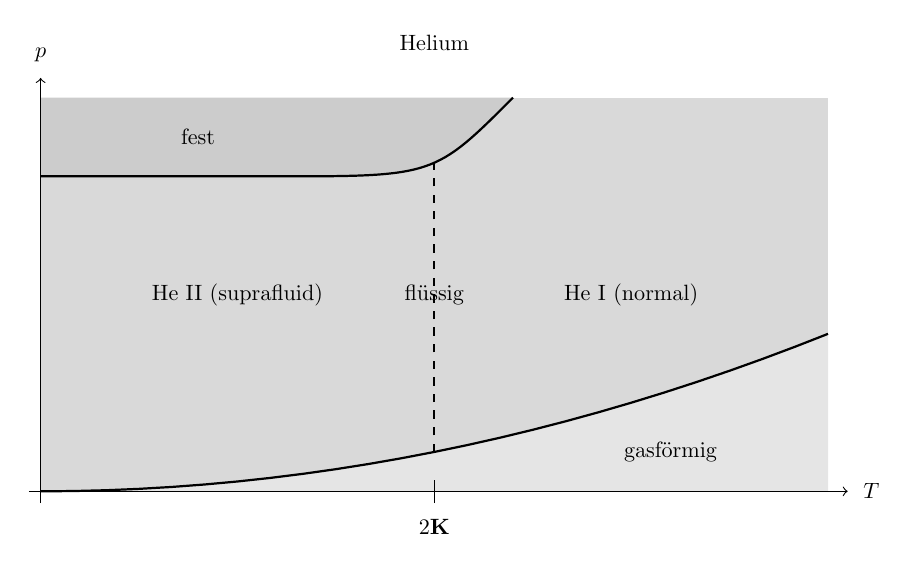
\begin{tikzpicture}[baseline=2.5cm]

  \fill[white!85!black] (0,0) rectangle (10,5);

  \draw[dashed,thick] (5,0.5) to (5,5);

  \fill[white!90!black,domain=0:10] (0,0) -- plot (\x,{(\x^2)/50}) -- (10,2) -- (10,0) -- cycle;

  \fill[white!80!black] (0,4) -- (3,4) .. controls (5,4) .. (6,5) -- (0,5) -- cycle;


  \draw[->] (0,-0.15) to (0,5.25);
  \draw[->] (-0.15,0) to (10.25,0);
  \node[anchor=south] at (0,5.35) {$p$};
  \node[anchor=west] at (10.35,0) {$T$};

  \draw[thick,domain=0:10] plot (\x,{(\x^2)/50});
  \draw[thick] (0,4) -- (3,4) .. controls (5,4) .. (6,5);

  \draw (5,-0.15) to ++ (0,0.3);
  \node[anchor=north] at (5,-0.25) {$2\textbf{K}$};

  \node[anchor=south] at (5,5.5) {\uline{Helium}};

  \node at (2,4.5) {fest};
  \node at (5,2.5) {flüssig};
  \node at (8,0.5) {gasförmig};

  \node at (2.5,2.5) {He II (suprafluid)};
  \node at (7.5,2.5) {He I (normal)};

\end{tikzpicture}
